%----------------------------------------------------------------------------
\chapter{Felhasználási lehetőségek}\label{sect:felhasznalas}
%----------------------------------------------------------------------------

A tekintet megfelelő minőségű és robusztus követésének számos gyakorlati felhasználása lehetséges. Elég csak a kutatási területek közül a \emph{perceptuális} (észlelési), vagy \emph{kognitív} (megértési) területekre gondolni, ahol például az olvasás, vagy az alvás folyamatának vizsgálatánál bizonyulhat hasznosnak.

Nem feltétlenül kell azonban a tekintetkövetést laboratóriumok falai közé szorítani: a rendszer számos gyakorlati életből vett felhasználási területen bizonyulhat hasznosnak, például a webergonómia vagy a vezetésbiztonság területein.

\bigskip

Az előző bekezdésekben felvázolt felosztás alapján a fejezet \sectref{tudomanyos} szakaszában a kutatási, míg a \sectref{gyakorlati} szakaszban a gyakorlati felhasználási lehetőségekről nyújtok egy vállaltan nem teljes körű, sokkal inkább az érdeklődés felkeltését célzó összefoglalást.

%,,,,,,,,,,,,,,,,,,,,,,,,,,,,,,,,,,,,,,,,,,,,,,,,,,,,,,,,,,,,,,,,,,,,,,,,,,,,
\section{Kutatási felhasználás}\label{sect:tudomanyos}
%,,,,,,,,,,,,,,,,,,,,,,,,,,,,,,,,,,,,,,,,,,,,,,,,,,,,,,,,,,,,,,,,,,,,,,,,,,,,

%............................................................................
\subsection{Kognitív pszichológia}\label{sect:kognitiv}
%............................................................................

A \textbf{kognitív} (megértési) pszichológia az egyik olyan kutatási terület, amelyben a tekintetkövetés igencsak hasznos eszköz lehet, hiszen a tudományág azt vizsgálja, hogy az ember hogyan látja a világot maga körül, és milyen módon képezi le azt.

\bigskip

Csak egy a lehetséges számtalan megértési probléma közül az \textbf{olvasási folyamat} működésének analízise. Az írott szöveg megértése összetett feladat, ennek a képességnek a hiánya egy tanulási részképességzavar, a \emph{diszlexia} meglétét jelentheti. A diszlexiás állapot felismerésében, a diagnózis megerősítésében, vagy akár az okok felkutatásában lehet hasznos eszköz a tekintetkövető rendszer.

\begin{figure}[!ht]
\centering
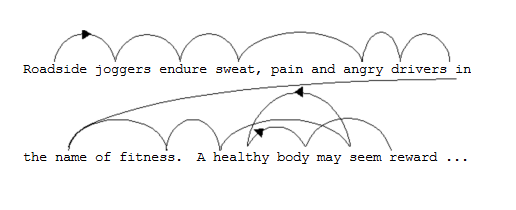
\includegraphics[width=100mm, keepaspectratio]{figures/read_saccade.png}
\caption{Szakkádok olvasás közben.\\Forrás: \url{http://bit.ly/C1ia}}
\label{fig:read_saccade}
\end{figure}

Lehetővé válhat a tekintet szakkadikus (egyszerűsítve: a tekintet trajektóriája, részletesen lásd \sectref{szakkadok} szakasz) mozgásának kellően gyors és pontos rögzítése, amely segítségével következtethetünk a megértési folyamat működésére, vagy éppen a működés hibáira. 

\bigskip

Alvásvizsgálat terén leginkább -- nevéből adódóan -- a REM (Rapid Eye Movement) fázis kötődik a szemmozgás követéséhez, ebben az alkalmazásban azonban értelemszerűen optikai elvű követés nem jöhet szóba.

%............................................................................
\subsection{Érzelemdetektálás}\label{sect:erzelem}
%............................................................................

A pupillaátmérő nem csak a fénymennyiség-változás hatására módosulhat. Érzelmi, izgalmi állapotok is előidézőik a változást, mint például félelem, idegesség vagy öröm \cite{altpszicho}. Ez a jelenség szintén potenciális felhasználási lehetőségeket rejt magában. Mivel a pupillareflex akaratlagosan nem koordinálható, állandó fénymennyiség mellett a pupillaméret változásának figyelésével detektálhatóvá válhatnak a fent említett érzelmi állapotok. Ehhez a változás mértékének és sebességének pontos mérése szükséges, ami azonban kellően nagy sebességű kamerával és elfogadható számítási teljesítményt nyújtó hardverrel kielégítő minőségben megtehető lehet. Az alkalmazás ráadásul nem feltétlenül igényli a szem közvetlen közelről (például fejre erősített kamerával) történő felvételét. Megfelelően nagy felbontású forrás esetén az arc-, majd szemrégió automatikus szegmentálása után a felismert zónát felhasználva, akár távolról is történhet a pupillareflex vizsgálata.

%............................................................................
\subsection{Orvosi felhasználás}\label{sect:orvosi_felh}
%............................................................................

Egyes betegségek is okozhatják a pupilla rendellenes méretét vagy viselkedését. Például a ,,miosis'', azaz a szem összehúzódása nemcsak a fent említett okokra vezethető vissza. Rendellenes összehúzódás alakulhat ki bizonyos patológiai állapotok, gyógyszerek, vagy mérgek hatására, sõt a mikrohullámú sugárzásnak kitett szervezet is produkálja ezt a tünetet. A ,,mydraisis'' (a pupilla tágulása) során ugyancsak nem megszokott viselkedés alakulhat ki bizonyos gyógyszerek vagy kábítószerek használatakor, de akár komoly fizikai trauma hatására is a normálisnál jelentősebb mértékű vagy időtartamú lehet a pupilla tágulata. A két szem eltérő méretű pupillája (az ,,anisocoria'') olyan betegségek meglétét jelezheti, mint a Horner-, vagy az Adie-szindróma \cite{altpszicho}. Orvosi szempontból is van tehát mit vizsgálni: a pupilla követésével egyes betegségek, állapotok felismerése, vagy alakulásuk megfigyelése laikus és orvos számára is automatizálható, megkönnyíthető lehet.

\bigskip

Továbbra is orvosi területen maradva a szemmozgás követése és regisztrálása \emph{ontoneurológiai} vizsgálatokban is szerepet kaphat. Az ilyen vizsgálat célja az egyensúlyszerv működésének megfigyelése és értékelése. Az összetett vizsgálat egyes fázisaiban a szemmozgások követése fontos információt hordoz az alany állapotáról, ugyanis a szemmozgató és az egyensúlyi információkat szállító idegpályák szoros kapcsolatban állnak egymással.

%,,,,,,,,,,,,,,,,,,,,,,,,,,,,,,,,,,,,,,,,,,,,,,,,,,,,,,,,,,,,,,,,,,,,,,,,,,,,
\section{Gyakorlati felhasználás}\label{sect:gyakorlati}
%,,,,,,,,,,,,,,,,,,,,,,,,,,,,,,,,,,,,,,,,,,,,,,,,,,,,,,,,,,,,,,,,,,,,,,,,,,,,

%............................................................................
\subsection{Webergonómia}\label{sect:webergonomia}
%............................................................................

Az ergonómia tudománya az ember és technika kapcsolatával, ezen belül is leginkább az említett kapcsolat zökkenőmentesítésével foglalkozik. 

Az ergonómia interdiszciplináris tudomány: egy ága a kapcsolat fizikai valójával foglalkozik (pl. kényelem, akadálymentes használat), egy másik terület inkább a pszichológiával rokonítható módon a fizikailag nem létező (virtuális) felhasználói felületek analízisével foglalkozik. Ugyancsak a grafikus felületek -- azon belül kifejezetten a weboldalak -- analízisével foglalkozik a manapság igencsak felkapott \emph{webergonómia} területe.

\begin{figure}[!ht]
\centering
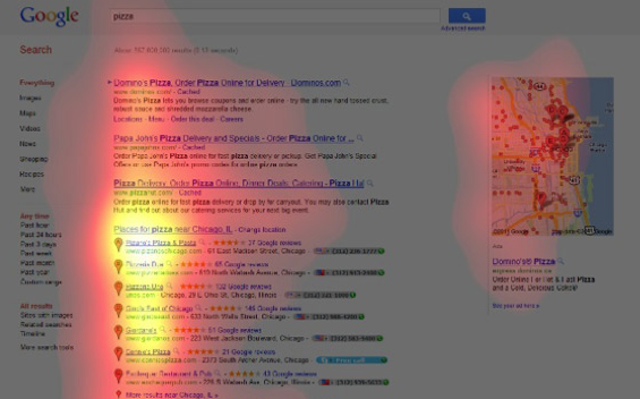
\includegraphics[width=100mm, keepaspectratio]{figures/google_heatmap.png}
\caption{A Google találati oldalának hőtérképes elemzése.\\Forrás: \url{http://on.mash.to/tHo2ap}}
\label{fig:google_heatmap}
\end{figure}

A megfelelő webes tervezés a \emph{felhasználói élmény} (user experience -- UX) szempontjából döntő fontosságú. Az elhelyezett tartalmak (legyen szó egy egyszerű honlapról, vagy egy összetett webalkalmazásról) közti navigációt úgy kell mind grafikailag, mind strukturálisan megtervezni, hogy a felhasználó intuitívan tudja használni a felületet.

Kellően pontos tekintetkövetéssel vizsgálható lehet, hogy a tervezés során mennyire sikerült a felhasználók igényeinek megfelelő felületet alkotni: könnyen eligazodnak-e rajta, esetleg idejük nagy részét a hibás tervezési döntések következtében kaotikus bolyongással töltik.

A felhasználói aktivitás rögzítésének felhasználására jó példa a \figref{google_heatmap} ábrán látható hőtérképes megjelenítés, amely a Google találati oldalának elemzésével támpontot nyújthat a keresőoptimalizálással foglalkozó szakemberek számára.

%............................................................................
\subsection{Vezetésbiztonság}\label{sect:orvosi_felhasznalas}
%............................................................................

Bár folynak már kutatások és tesztek vezető nélküli, automatizált járművek közúti használatára\footnote{például \emph{Google Driverless Car}, lásd \url{http://bit.ly/PehN2r}}, a humán faktor valószínűleg még nagyon sokáig nem lesz teljesen megkerülhető, ha autóvezetésről van szó.

Vezetésbiztonsági alkalmazásban is elképzelhető lehet a tekintetkövetés alkalmazása. A vezető fókuszának vizsgálatán túl, a követés során mintegy járulékos információként mérhetjük a pislogások gyakoriságát és hosszát is, ezzel felismerhetővé válhat a gépjárművezetés közben lankadó figyelem, és jelezhető, ha fennáll az elalvás veszélye. Az eljárás így hasznosnak bizonyulhat már meglévő elalvásdetektálási módszerek \cite{sleepdet} kiegészítéseként, tovább javítva azok megbízhatóságát.

\begin{figure}[!ht]
\centering
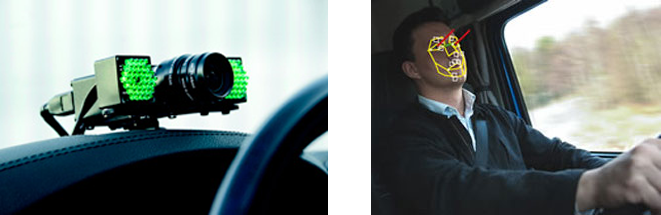
\includegraphics[width=100mm, keepaspectratio]{figures/driving.png}
\caption{\textbf{Bal:} A \emph{Daimler} tekintetkövető kamerája. \\ Forrás: \url{http://bit.ly/14jX6I2} \\
\textbf{Jobb:} A \emph{Seeing Machines} DSS nevű megoldása. \\ Forrás: \url{http://bit.ly/16HLaDE}}
\label{fig:driving}
\end{figure}

%,,,,,,,,,,,,,,,,,,,,,,,,,,,,,,,,,,,,,,,,,,,,,,,,,,,,,,,,,,,,,,,,,,,,,,,,,,,,
\section{Összefoglalás}\label{sect:felh_osszefoglalas}
%,,,,,,,,,,,,,,,,,,,,,,,,,,,,,,,,,,,,,,,,,,,,,,,,,,,,,,,,,,,,,,,,,,,,,,,,,,,,

\texttt{+++ par mondatos osszefoglalas +++}